\section{Cifrado César}
Tal como se pide, se realiza un algoritmo para el descifrado mediante el comando \texttt{tr} del bash. Para ello se realiza un pequeño script, el cual permitirá pasar la cadena cifrada directamente al momento de ejecutar el comando, es decir de la forma: 
\begin{verbatim}
	cesar\_descifrar.sh [texto_a_descrifrar]
\end{verbatim}

Cuando el archivo se le hayan dado permisos de ejecución (\texttt{chmod +x cesar\_descifrar}), el algoritmo convertirá toda la cadena en minúsculas, para luego aplicar César (desplazamiento de letras) a la cadena. Esto lo iterará e imprimirá para todas las 26 letras del abecedario (sin ñ).

\begin{lstlisting}[language=bash]
#!/bin/bash
alfabeto="abcdefghijklmnopqrstuvwxyz"

# Validamos que el usuario haya proporcionado un argumento
if [ -z "$1" ]; then
echo "Modo de uso:"
echo "$0 [cadena_a_descifrar]"
exit 1
fi

# El argumento posicional se asigna a la variable, traduciendolo a minusculas
cadena=$(echo "$1" | tr 'A-Z' 'a-z')

# Iteracion de rotaciones de letras
echo "-----------------------------------"
echo "Aplicando fuerza bruta a: $cadena"
for i in {1..25}; do
desplazamiento="${alfabeto:$i}${alfabeto:0:$i}"
descifrado=$(echo "$cadena" | tr "$alfabeto" "$desplazamiento")
echo "$i: $descifrado"
done
\end{lstlisting}
De esta forma probamos todas las cadenas a encriptar. A continuación se muestra la ejecución del script con la primera cadena:
\begin{figure}[H]
	\centering
	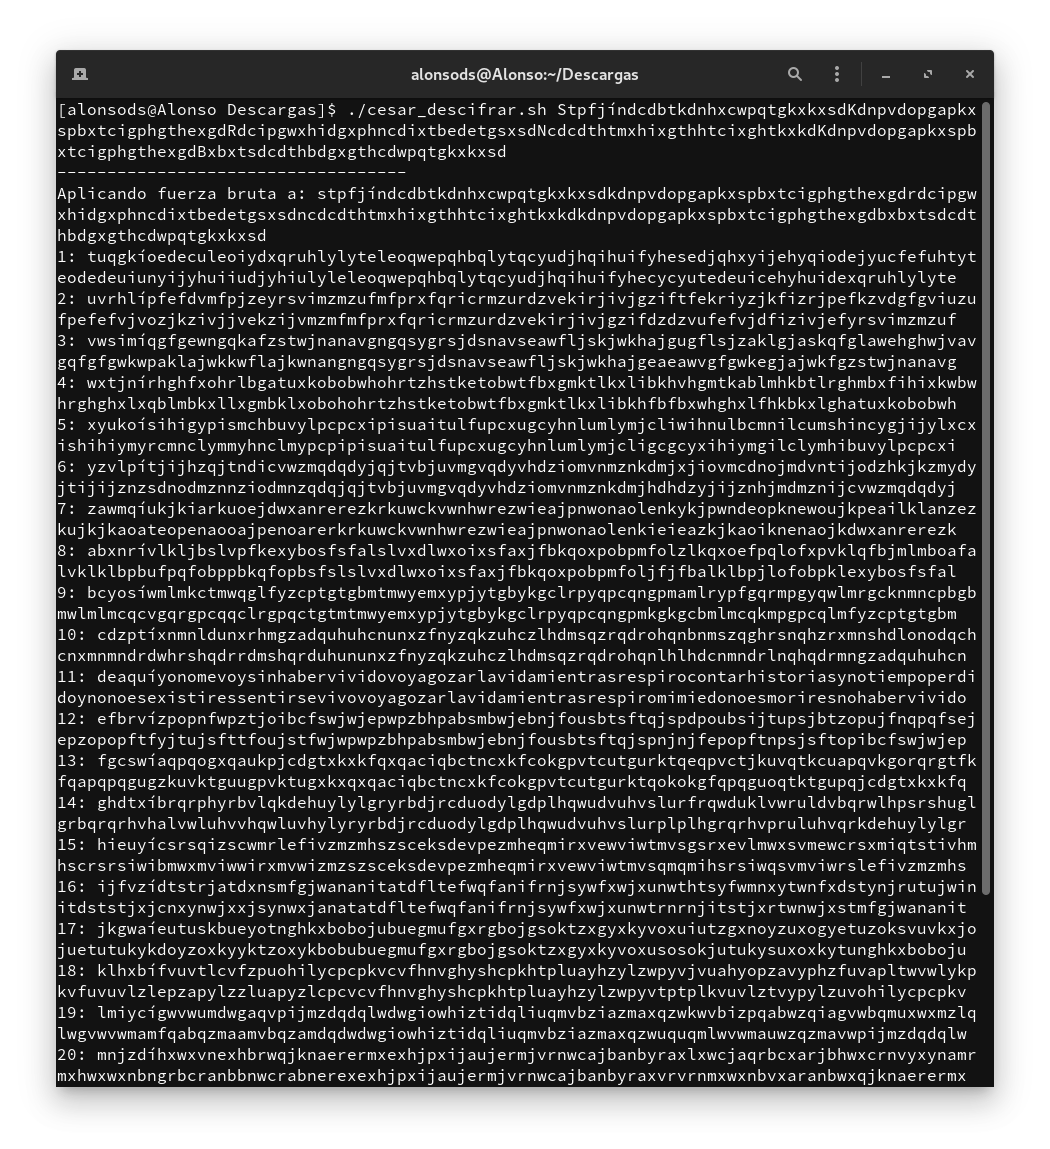
\includegraphics[scale=0.4]{imagenes/Capturas/1.png}
	\label{fig:ipCentralOps}
\end{figure}

Se realizó el script para todas las cadenas, tras una cuidadosa observación, se lograron descifrar algunos textos. A continuación se muestran solo las cadenas descifradas (en César).
\begin{itemize}
	\item \textbf{Cadena 1 (descifrada):}
	\begin{verbatim}
		deaquíyonomevoysinhabervividovoyagozarlavidamientrasrespirocontarhistoriasyno
		tiempoperdidoynonoesexistiressentirsevivovoyagozarlavidamientrasrespiromimiedo
		noesmoriresnohabervivido
	\end{verbatim}
	\item \textbf{Cadena 6 (descifrada):}
	\begin{verbatim}
		mayyouhaveauspiciousnessandcausesofsuccessmayyouhavetheconfidencetoalways
		doyourbestmayyoutakenoeffortinyourbeinggeneroussharingwhatyoucannothing
		morenothinglessmayyouknowthemeaningofthewordhappinessmayyoualwayslead
		fromthebeatinginyourchestmayyoubetreate
	\end{verbatim}
	\item \textbf{Cadena 9 (descifrada):}
	\begin{verbatim}
		lavidaesunpocovilescorrectoolvídateyadeabrilniqueestuvieraenlatínnotemoa
		fracasarsiemprehesidoeldeatráselúnicofracasoesnotratarnotemoafracasar
		nihallegarhastaelfinalloúnicoesquesemeacabaelgas
	\end{verbatim}
\end{itemize}

\section{Cifrado Vigenère}
Tal como se propone para Vigenère, se creó un programa en Python para la desencriptar las cadenas fácilmente. Para ello, se nos proporcionan las llaves de descifrado \textit{star, pinamar, lazy, lagrima, passenger, diente}, por lo cual usaremos estas palabras para nuestro diccionario de llaves. El programa capturará la cadena a desencriptar, para luego imprimir sus resultados de aplicar el algoritmo de Vigenère con cada una de las llaves.
El programa implementa el algoritmo desencriptación de Vigenère con la función \texttt{descifrar\_vigenere}, el cual funciona de la siguiente manera:
\begin{itemize}
	\item Al inicio, declaramos nuestras variables de interés que utilizaremos para el algoritmo: texto a cifrar, la llave, el texto descifrado y el índice de iteración.
	\item Para aplicar las operaciones del cifrado, es necesario que las letras del alfabeto correspondan a los valores numéricos del 0 al 25. Aunque este "mapeo" se puede realizar manualmente con un \texttt{match}, utilizaremos el valor ASCII que ya poseen todas las letras. Esto se hará con la función \texttt{ord()}.
	\item Aplicamos la fórmula matemática de desencriptación:
	\begin{equation}
		p_i = (c_i - k_i + 26) % 26
	\end{equation}
	donde $p_i$ es la i-ésima letra del texto descifrado, $c_i$ es la i-ésima letra del texto cifrado, y $k_i$ es la i-ésima letra de la llave.
	\item Vigenère requiere que la llave se repita cíclicamente a lo largo de todo el texto. Para lograr esto, se utiliza el operador módulo sobre la longitud de la llave: \texttt{indice\_llave \% len(llave)}.
	\item El valor númerico de $p_i$ se convierte a su carácter ASCII correspondiente aplicandole la función \texttt{chr()}.
\end{itemize}
\begin{lstlisting}[language=Python]
#!/usr/bin/env python3

def descifrar_vigenere(texto_cifrado, llave):
texto_cifrado = texto_cifrado.lower()
llave = llave.lower()
texto_descifrado = ""
indice_llave = 0

for caracter in texto_cifrado:
if 'a' <= caracter <= 'z':
# Convertimos las letras a valores de 0 a 25
c_i = ord(caracter) - ord('a')
k_i = ord(llave[indice_llave % len(llave)]) - ord('a')

# Aplicamos la fórmula matemática del descifrado
p_i = (c_i - k_i + 26) % 26

# Regresamos el valor a su representación ASCII
texto_descifrado += chr(p_i + ord('a'))

# Solo avanzamos el índice de la llave si procesamos una letra
indice_llave += 1
else:
# Preservamos espacios y puntuación
texto_descifrado += caracter

return texto_descifrado

# Diccionario de llaves a iterar
llaves_candidatas = ["star", "pinamar", "lazy", "lagrima", "passenger", "diente"]

print("=== Descifrador Vigenère por Ataque de Diccionario ===")
print("Ingresa una cadena vacía (presiona Enter sin escribir nada) para salir.\n")

while True:
try:
# Capturamos la entrada estándar y limpiamos espacios en blanco a los lados
cadena = input("Ingresa la cadena cifrada: ").strip()

# Condición de salida: cadena vacía
if not cadena:
print("Cadena vacía detectada. Terminando el programa...")
break

print("\n--- Resultados ---")
for llave in llaves_candidatas:
resultado = descifrar_vigenere(cadena, llave)
print(f"Llave '{llave}': {resultado}")
print("-" * 40 + "\n")

except (EOFError, KeyboardInterrupt):
# Captura Ctrl+D o Ctrl+C para una salida limpia en la terminal
print("\nTerminando el programa...")
break
\end{lstlisting}
En cuanto al flujo del programa, se implementó un ciclo \texttt{while True} que captura la entrada de cadenas continuamente. Detiene su ejecución al detectar una cadena vacía o una señal de interrupción del sistema, e itera de forma automática sobre la lista predefinida de 6 llaves del diccionario.
Se ejecuto el programa con las cadenas restantes que no se reolvieron con César. Tras una cuidadosa observación, se lograron descifrar estos textos restantes. A continuación se muestran las cadenas descifradas (con Vigenère):
\begin{itemize}
	\item \textbf{Cadena 2 (descifrada)} con llave \texttt{pinamar}:
	\begin{verbatim}
		fueunveranoenpinamarsinnecesidaddeconversaryempujadosporelvientosedetuvo
		eltiempoenunbalconconvistaalmarfueunveranoenpinamarcondenadoalaeternidad
		yapasarontantosanosysigorecordandolanocheenpinamar
	\end{verbatim}
	\item \textbf{Cadena 3 (descifrada)} con llave \texttt{passenger}:
	\begin{verbatim}
		butyouonlyneedthelightwhenitsburninglowonlymissthesunwhenitstartstosnow
		onlyknowyouloveherwhenyoulethergoonlyknowyouvebeenhighwhenyourefeeling
		lowonlyhatetheroadwhenyouremissinghomeonlyknowyouloveherwhenyoulether
		gostaringattheceilinginthedarksameoldemptyfeelinginyourheart
	\end{verbatim}
	\item \textbf{Cadena 4 (descifrada)} con llave \texttt{lazy}:
	\begin{verbatim}
		todayidontfeellikedoinganythingijustwannalayinmybeddontfeellikepickingup
		myphonesoleaveamessageatthetonecausetodayiswearimnotdoinganythingim
		gonnakickmyfeetupthenstareatthefanturnthetvonthrowmyhandinmypants
	\end{verbatim}
	\item \textbf{Cadena 5 (descifrada)} con llave \texttt{diente}:
	\begin{verbatim}
		siemprefuisteelmasblancoelquenuncatuvosarronotuvistepicadurasniunasola
		carieyahorasinprevioavisotesoltasteyanomasticasnadacomoantesbrillabas
		cuandosonreiaymascabamospastillasnoscomimosmilcostillassopaipillascon
		pureahoranotriturasnadanomuerdeslechenevadatalvezseaculpamiadime
		dientedimelo
	\end{verbatim}
	\item \textbf{Cadena 7 (descifrada)} con llave \texttt{lagrima}:
	\begin{verbatim}
		enmipancitarevoloteanmaripositasdeprimaveraestoynerviosoestoy
		temblandocreomeestoyenamorandoquierodecirteunacositaqueeresmuy
		lindaymuybonitayanomesalenlaspalabrastengounnudoenlagargantanote
		imaginasloquemueroporsabersituminoviaquieresserhacetiempoqueno
		comoyquenoduermoporquetumiradasequedaclavadaenmimentedesde
		elprimerdiaquetevi
	\end{verbatim}
	\item \textbf{Cadena 8 (descifrada)} con llave \texttt{star}:
	\begin{verbatim}
		thatnowourdreamstheyvefinallycometruecityofstarsjustonethingevery
		bodywantsthereinthebarsandthroughthesmokescreenofthecrowded
		restaurantsitsloveyesallwerelookingforislovefromsomeoneelsearusha
		glanceatouchadance
	\end{verbatim}
\end{itemize}

\section{Prueba de IA}
Se le proporciono a ChatGPT el cuarto texto encriptado. Estas fueron las pistas que le fueron brindadas hasta que consiguió encontrar la llave correcta.
\begin{itemize}
	\item El idioma del mensaje está en inglés.
	\item El cifrado es Vigenère y la longitud de la clave es 4.
	\item El mensaje original empieza con una palabra de 5 letras.
	\item El mensaje original contiene la subcadena IM-GONNA-KICK-MY-FEET.
	\item El texto original tiene 57 palabras, con solo 2 contracciones IM.
\end{itemize}
En este punto, la mayoría de los textos desencriptados que daba eran textos ilegibles (y por ende, incorrectos). Pocas veces, dio como respuesta un texto legible, sin embargo no era el texto original. No comprendó bien como los obtuvo.
Después de dar todas las pistas anteriores, sugirió que la clave era \textbf{azyl}, que justamente es una permutación de la clave correcta (\textbf{lazy}), lo cual me sorprendió que la secuencia era correcta, solo el orden no lo era. Le siguieron las siguientes pistas:
\begin{itemize}
	\item La clave correcta tiene todas las letras de la última clave descubierta.
	\item La clave también es una palabra en inglés.
\end{itemize}
Fue así como encontró la clave correcta, sin embargo, sorprendentemente aún con tener la clave correcta, dió un texto desencriptado totalmente diferente. Le indiqué que el texto no era correcto y que calculara nuevamente con cuidado. \\
Finalmente, encontró el texto descifrado correcto después de un tiempo de procesamiento notablemente mayor (el más alto) al de el resto de peticiones. Se anexa el chat: \\
\url{https://chatgpt.com/share/69abbcf2-6b54-8004-b194-7083fb5cfb86}